\chapter{Systembeskrivelse}

Overordnet set består systemet af en hardware- og en software-del. Hardwaren er blevet udleveret og består af DAQ og Analog-discovery. DAQ'en og Analog-discovery har begge forbindelse til computeren som har forbindelse til hinanden, se figur 4.1.  

\begin{figure}[H]
	\centering
	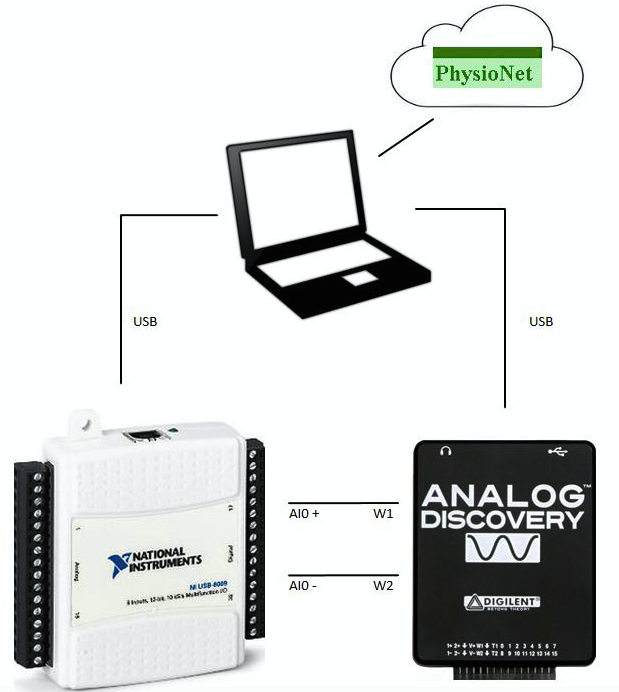
\includegraphics[width=0.8\textwidth]{Figurer/Snip20150427_1}
	\caption{Opstilling af Hardwaren}
\end{figure}

I projektet analyseres virtuelle patienters EKG-signaler. Disse EKG-signaler kommer fra PhysioNet, som er ekstern database, der kan tilgås via internettet\footnote{www.physionet.org}. EKG-signalet, der ønskes analyseres hentes ned som en CSV-fil. Filen's information bliver omdannet til et analog signal, som simuleres af Analog-discovery. Det analoge signal bliver konverters til et digtital signal af DAQ'en. Det er det digitale signal systemet kan afbillede og analysere.   


Systembeskrivelsen er en kort beskrivelse af det samlede system der er tænkt realiseret i projektet. Systembeskrivelsen bør indeholde en illustration eller et diagram af systemet.
Beskrivelsen bør ligeledes fortælle, om systemet er bygget som en prototype eller et ende- ligt produkt. Brug fotos af opstillingen.



Overordnet set, består systemet af en hardware del, og en softwaredel. Hardwaredelen er udleveret, og vil derfor ikke blive beskrevet i dybden. Den del af systemet, som reelt set er prototypen, er derimod softwaren, som er udviklet i gruppen. Hvis der er interesse for yderligere kommentarer vedrørende hardwaren, henvises der til afsnittet ’Hardware-arkitektur’ i dokumentationen.